\section{Performance Tests}
\label{sec:performance}


\subsection{Methods}
\label{sec:performance:methods}

In this section, we briefly describe the technical means by which we were able to test the relative performance of GeoWave and GeoMesa for indexing \texttt{SimpleFeature}s in Accumulo.

The ultimate aim of the method of deployment, ingesting, and running the tests was to ensure results were both repeatable and could be iterated on quickly.
This implies these methods and the associated software are useful beyond the needs of this comparative analysis.
All software associated with the performance tests is open sourced under the Apache 2.
license, and can be found at \url{https://github.com/azavea/geowave-geomesa-comparative-analysis}.


\subsection{Environment}
\label{sec:performance:environment}

For all deployments, the software versions shown in Table \ref{table:software} were used:

\begin{table}[h!tb]
  \centering
  \begin{tabular}{ | l || c | c | c | c | c | c | }
    \hline
    Software & Hadoop & Spark & Zookeeper & Accumulo & GeoMesa & GeoWave \\ \hline
    Version  & 2.7.2  & 2.0.0 & 3.4.8 & 1.7.2 & 1.2.6 & 0.9.3-SNAPSHOT \\
    \hline
  \end{tabular}
  \caption{Software versions.}
  \label{table:software}
\end{table}

For GeoWave, we used a snapshot version based on the code that can be found at commit SHA \texttt{8760ce2cbc5c8a65c4415de62210303c3c1a9710}.

Across all tests, Amazon Web Service (AWS) Elastic Cloud Compute (EC2) instances were used.
The machine types used are displayed in Table \ref{table:machines}.

\begin{table}[h!tb]
  \centering
  \begin{tabular}{ | l | c | c | c | c | }
    \hline
    & Instance Type & vCPU & Mem (GB) & Storage (Drives x GB) \\ \hline
    Query Server & \texttt{m3.large} & $2$ & $7.5$ & $1\times32$ \\
    Cluster Master & \texttt{m3.xlarge} & $4$ & $15$ & $2\times40$ \\
    Cluster Worker & \texttt{m3.2xlarge} & $8$ & $30$ & $2\times80$ \\
    \hline
  \end{tabular}
  \caption{Amazon machine types.}
  \label{table:machines}
\end{table}

\subsection{Deployment}
\label{sec:performance:deployment}

A minimal working environment for either GeoWave or GeoMesa (assuming, as we do, an Accumulo backend) includes a number of interdependent, distributed processes through which consistent and predictable behavior is difficult to attain.
Each of these pieces - i.e. Apache Zookeeper, HDFS, Accumulo - is a complex bit of technology in and of itself. Their interoperation multiplies this complexity and introduces the race conditions one expects of distributed systems.

The solution to repeatability under this complexity that we arrived at was to develop a set of Docker containers which jointly provide the pieces necessary to bring up GeoWave and/or GeoMesa on top of Accumulo.
A system of deploying the necessary components, which exists under the name GeoDocker, was improved to the point that we could consistently deploy Accumulo with the necessary components for GeoMesa and GeoWave to identical Hadoop clusters on Amazon Web Service's (AWS) Elastic Map Reduce (EMR).
We opted to use the YARN, Zookeeper, and HDFS which is distributed on Amazon EMR to support GeoDocker’s Accumulo processes.

Pictured in Figure \ref{deployment} is a rough diagram of the deployment used throughout our efforts.

\begin{figure}[h!tb]
  \centering
  \includegraphics[width=0.60\textwidth]{../docs/img/test-environment-architecture.png}
  \caption{Test environment architecture.}
  \label{deployment}
\end{figure}

The entire infrastructure for running queries and collecting timings results ran as a set of REST endpoints, created using the akka-http project.
Each endpoint represented a different test case, and timing results were taken from inside of the application to only measure GeoWave and GeoMesa performance.
Results were saved off to an AWS DynamoDB table for analysis, and included information about the duration of the query, the timing to the first result of the query, and cluster configuration information.
These query servers ran on AWS Elastic Container Service, and all query servers all sit behind an AWS load balancer to allow for multitenancy testing.


\subsection{Ingest}
\label{sec:performance:ingest}

All data used for benchmarking these systems was loaded through custom Spark-based ingest programs.
Initial attempts to use the command line tools provided by each of the projects were met with a few notable difficulties; this made writing our own ingest programs the simplest solution.
Both teams were consulted about our ingest tooling to verify their correct operation.
Using our own version of ingest tooling has the disadvantage that ingest timing results cannot be considered in the comparative analysis; however we determined that our Spark-based tooling was the best path forward to provide consistent and successful ingests of our test datasets into both systems with exactly the same data.

See Appendix \ref{appendix:ingest}: Details of Ingest Tooling for a more complete description of the ingest tooling.

We recorded the size on disk, number of entries, tablet server information and other details for each dataset ingested.
These can be found in Appendix \ref{appendix:data}: Details of Ingested Data


\subsection{Querying}
\label{sec:performance:querying}

Queries were generated and submitted by the query servers in response to requests from clients.
This arrangement was chosen because it allowed for quick experimentation and prototyping of different parameters simply by tweaking requests while also ensuring that results were as reproducible as possible. Results generated for this report should be conveniently reproducible and decisions about which results should be generated, in what order, and how many times are largely configurable.

For a group of queries we will call the ``Serial Queries'' tests, the specific queries were run one at a time, so that the only load on the GeoWave or GeoMesa system was a single query.
For the ``Multitenancy Stress'' tests, a framework was used to produce a number of concurrent connections, so that we could test the multitenancy use case by querying the systems in parallel.


\subsection{Datasets}
\label{sec:performance:datasets}

We conducted performance tests on three different data sets, which are described below.

\subsubsection{GeoLife}
\label{sec:performance:datasets:geolife}

This GPS trajectory dataset was collected as part of the Microsoft Research Asia Geolife project by $182$ users in a period of over five years (from April 2007 to August 2012).
A GPS trajectory of this dataset is represented by a sequence of time-stamped points, each of which contains the information of latitude, longitude and altitude.
This dataset contains $17,621$ trajectories with a total distance of $1,292,951$ kilometers and a total duration of $50,176$ hours.
These trajectories were recorded by different GPS loggers and GPS phones, and have a variety of sampling rates.
$91.5$ percent of the trajectories are logged in a dense representation, e.g. every $1$ to $5$ seconds or every $5$ to $10$ meters per point.
Although this dataset is wildly distributed in over $30$ cities of China and even in some cities located in the USA and Europe, the majority of the data was created in Beijing, China.

Text taken from the GeoLife user guide, found at \url{https://www.microsoft.com/en-us/research/wp-content/uploads/2016/02/User20Guide-1.2.pdf}.


\subsubsection{GDELT}
\label{sec:performance:datasets:gdelt}

GDELT-Global Data on Events, Location and Tone is a new CAMEO-coded data set containing more than $200$ million geolocated events with global coverage for 1979 to the present.
The data are based on news reports from a variety of international news sources coded using the Tabari system for events and additional software for location and tone.
The data is freely available and is updated daily.
The GDELT data we have tested against contains data up through August 2016.

Text taken from the ISA 2013 paper introducing GDELT, found at \url{http://data.gdeltproject.org/documentation/ISA.2013.GDELT.pdf}.


\subsubsection{Synthesized Tracks}
\label{sec:performance:datasets:synthesized}

We tested against a dataset supplied by a third party that that contain a total of $6.34$ million synthesized tracks.
This set of tracks had a median length of $29.8$ km, a mean length of $38.82$ km and each track contains an average of $491.45$ points.
There was approximately $35.88$ GB of data compressed and stored as $729$ Apache Avro encoded files.
The tracks were generated through a statistical process using Global OpenStreetMap data and Global Landscan data as inputs.
The dataset is available at \url{s3://geotrellis-sample-datasets/generated-tracks/}.

Figure \ref{geoserver} is a view of the data for a specific time slice of the data, as shown in GeoServer.
Table \ref{table:lengths} gives a statistical summary of the dataset.

\begin{figure}[h!tb]
  \centering
  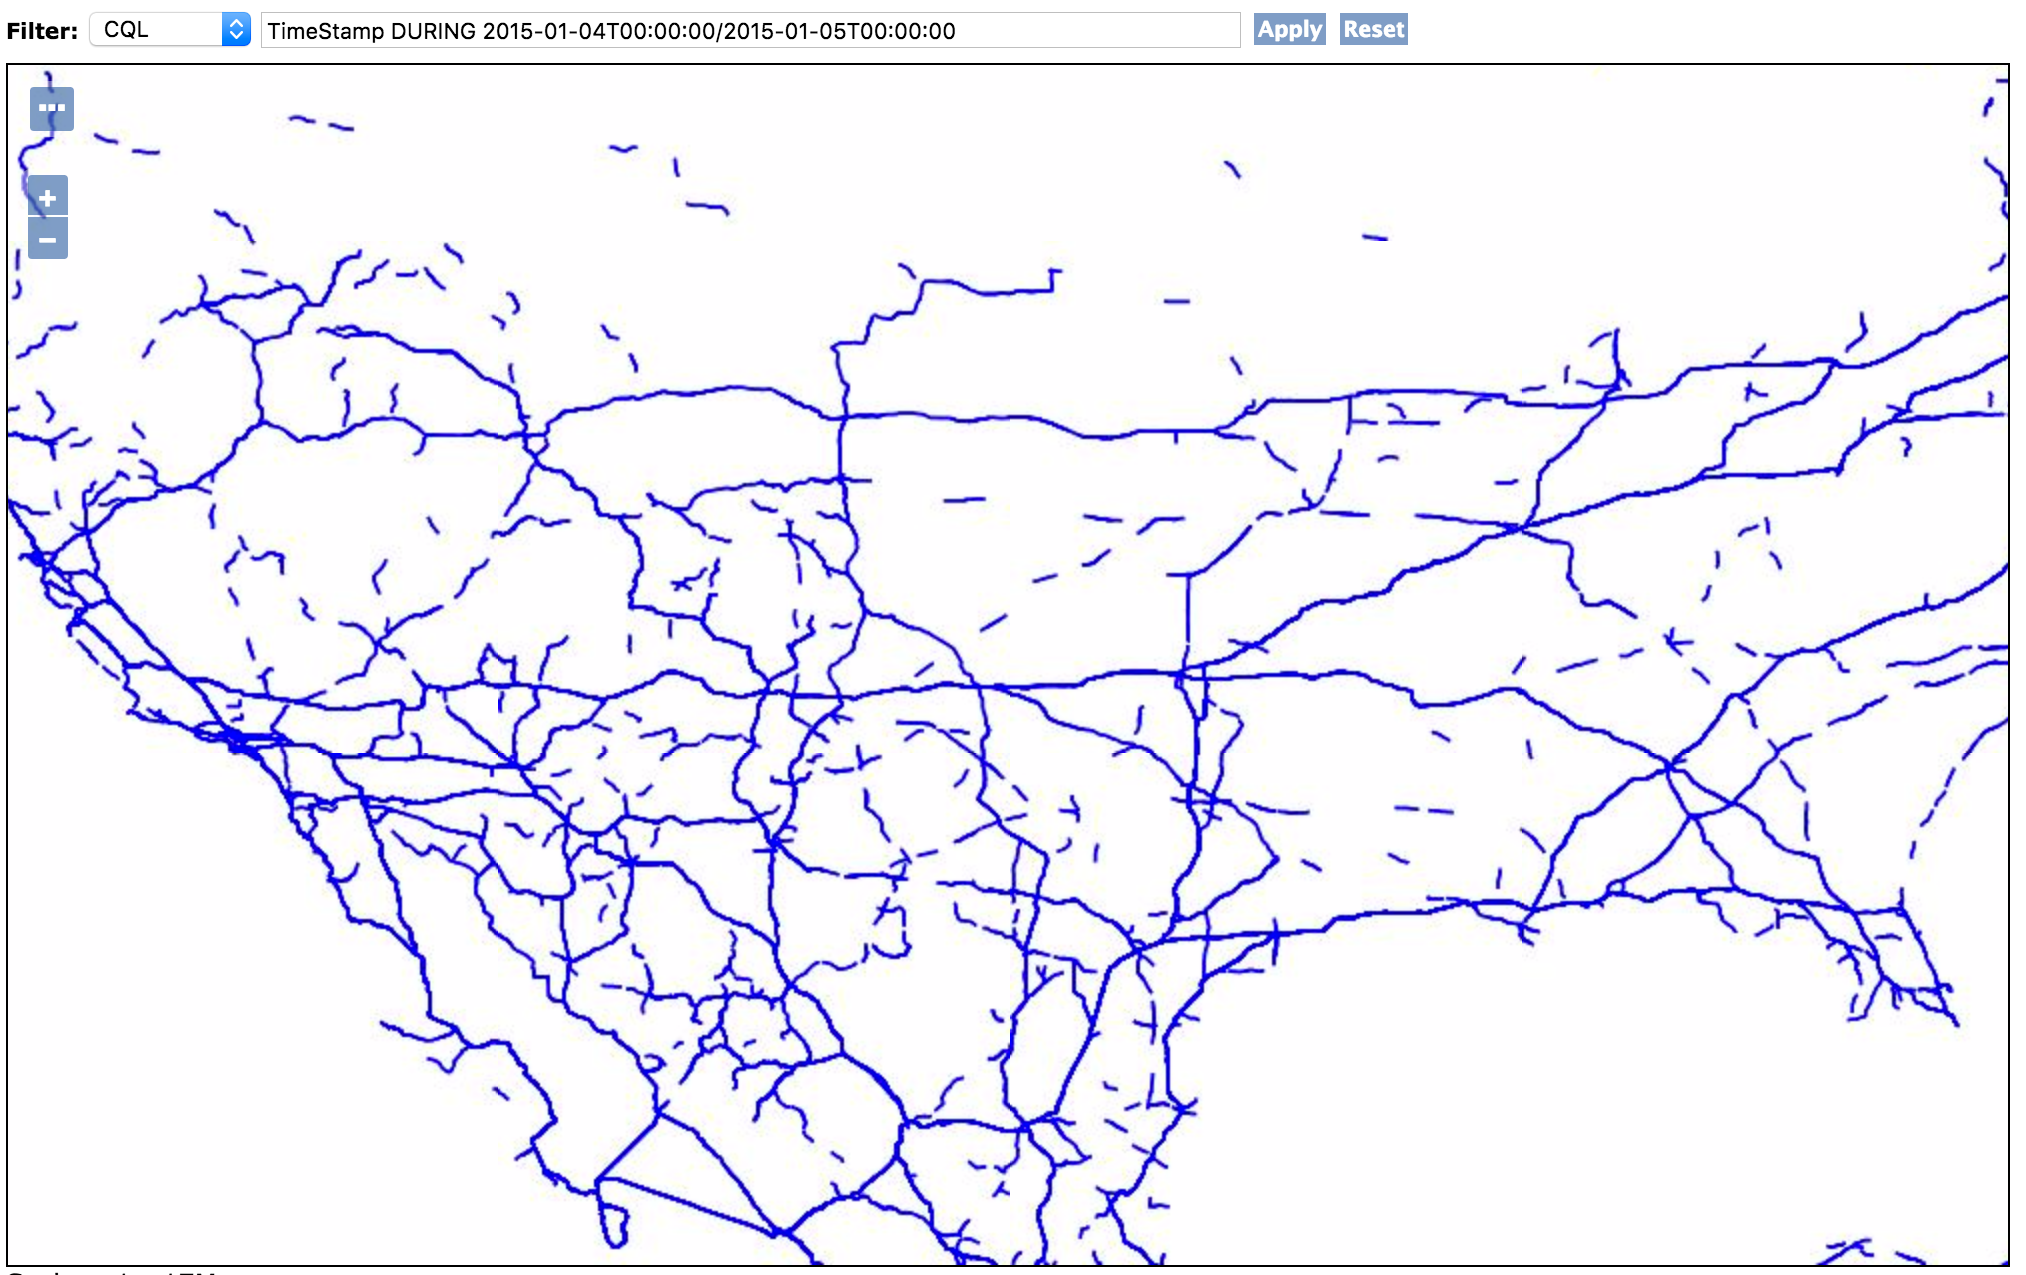
\includegraphics[width=0.60\textwidth]{../docs/img/tracks/synthetic-tracks.png}
  \caption{Synthetic Tracks}
  \label{geoserver}
\end{figure}

\begin{table}[h!tb]
  \centering
  \begin{tabular}{ | c | c | c | c | c | c | c | c | }
    \hline
    count & min & max & mean & std dev & median & skewness & kurtosis \\ \hline
    $2054751$ & $0.064998$ & $2839.198486$ & $38.829134$ & $115.975988$ & $29.791367$ & $15.466978$ & $266.782216$ \\
    \hline
  \end{tabular}
  \caption{Track Length Stats (in miles).}
  \label{table:lengths}
\end{table}
